% ============================================================
%  Chapter 5 -- System Implementation: Results and Discussion
% ============================================================

\subsection{Introduction}

This chapter documents the hardware realisation, software development, and validation testing of TAMRA (Task-Agnostic Modular Robotic Apparatus). The first semester established the design foundation. The second semester converted those decisions into a working system and required two course corrections that are explained before the technical content: a platform change, and a scope refinement.

% -------------------------------------
\subsection{Platform Selection: From TurtleBot to iMRP500}
% -------------------------------------

Semester one was spent studying TurtleBot~4 and iCreate~3 in simulation. That work was productive -- it built a solid foundation in ROS~2 \cite{macenski2022ros2}, SLAM, and sensor fusion that carried into implementation. When procurement time arrived, however, both platforms were ruled out.

iRobot, manufacturer of the iCreate~3, entered bankruptcy proceedings at the same time the team needed to commit a purchase \cite{irobot2024create3}. With a fixed budget and an eight-week deadline, depending on a platform with uncertain long-term support was not viable. TurtleBot~4 shares the same Create~3 base and carries the same risk.

Beyond sustainability, both platforms lack any engineered mounting interface for a body structure -- neither is designed to accept a tall shell, and improvised fixturing would have introduced mechanical instability incompatible with the physical design goals.

This platform transition proved to be a critical turning point. The alternative platforms discovered during the search were superior across every relevant dimension: payload capacity, onboard sensor integration, structural rigidity, and long-term vendor support. The switch was the difference between a system that could be realistically deployed in a service environment and one that would remain a laboratory prototype.

\subsubsection{The Service Robot Landscape}

Before selecting a platform, it was important to understand the broader ecosystem. Service robots divide into two fundamentally different categories: \textbf{ready-to-use robots} pre-configured for a specific industry vertical, and \textbf{chassis bases} that expose a raw navigation and sensor stack for a developer to build upon. Figure~\ref{fig:landscape} maps the ecosystem.

\begin{figure}[H]
\centering

% --- ROW 1 LABEL ---
\noindent\textbf{Chassis Bases} \hfill {\small (open platform, developer builds on top)}
\vspace{4pt}

\noindent
\begin{minipage}[t]{0.23\linewidth}\centering
  
\includegraphics[width=\linewidth,height=3.0cm,keepaspectratio]{plat_ciot.jpg}\\[3pt]
  {\small\textbf{iMRP500}\\
  \textit{Selected}\\
  850\,OMR incl.\ shipping}
\end{minipage}\hfill
\begin{minipage}[t]{0.23\linewidth}\centering
  
\includegraphics[width=\linewidth,height=3.0cm,keepaspectratio]{plat_wheeltec.jpg}\\[3pt]
  {\small\textbf{Wheeltec S100}\\
  \textit{ROS~1/2, academic}\\
  from 550\,OMR}
\end{minipage}\hfill
\begin{minipage}[t]{0.23\linewidth}\centering
  
\includegraphics[width=\linewidth,height=3.0cm,keepaspectratio]{plat_waterdrop.jpg}\\[3pt]
  {\small\textbf{Water Drop (Shuidi II)}\\
  \textit{Circular, 50\,kg payload}\\
  $\sim$\$2{,}285}
\end{minipage}\hfill
\begin{minipage}[t]{0.23\linewidth}\centering
  \vspace{0.6cm}
  {\small\textbf{Slamtec Series}\\
  SDP Mini \$500\\
  Apollo 2.0\\
  Hermes $\sim$\$2{,}000}
\end{minipage}

\vspace{10pt}
\noindent\rule{\linewidth}{0.3pt}
\vspace{6pt}

% --- ROW 2 LABEL ---
\noindent\textbf{Ready-to-Use Robots} \hfill {\small (closed software, industry-specific)}
\vspace{4pt}

\noindent
\begin{minipage}[t]{0.23\linewidth}\centering
  
\includegraphics[width=\linewidth,height=3.0cm,keepaspectratio]{plat_reception.jpg}\\[3pt]
  {\small\textbf{Reception / Guide}\\
  Touchscreen, face recognition\\
  No payload. Guides only.}
\end{minipage}\hfill
\begin{minipage}[t]{0.23\linewidth}\centering
  
\includegraphics[width=\linewidth,height=3.0cm,keepaspectratio]{plat_restaurant.jpg}\\[3pt]
  {\small\textbf{Restaurant Delivery}\\
  e.g.\ Keenon T5\\
  Open shelves, \$1{,}700--3{,}000}
\end{minipage}\hfill
\begin{minipage}[t]{0.23\linewidth}\centering
  
\includegraphics[width=\linewidth,height=3.0cm,keepaspectratio]{plat_hotel.jpg}\\[3pt]
  {\small\textbf{Hotel Delivery}\\
  Enclosed locking compartments\\
  PIN/QR access, elevator control}
\end{minipage}\hfill
\begin{minipage}[t]{0.23\linewidth}\centering
  
\includegraphics[width=\linewidth,height=3.0cm,keepaspectratio]{plat_factory.jpg}\\[3pt]
  {\small\textbf{Factory AMRs}\\
  100--1{,}000+\,kg payload\\
  Pallet lift, tow carts}
\end{minipage}

\caption{Service robot ecosystem. \textit{Top row}: chassis bases that expose open navigation APIs for developers to build on. \textit{Bottom row}: ready-to-use robots locked to a single industry vertical. Restaurant and hotel delivery robots are the most widely deployed service robot category globally. None of the ready-to-use categories offer an open interface for adding conversational AI, custom bodies, or research-level sensor access -- hence the chassis-base approach.}
\label{fig:landscape}
\end{figure}

\noindent The ready-to-use categories each serve a narrow purpose. Restaurant robots use open shelves and are optimised for crowded kitchen-to-table trips. Hotel robots carry enclosed locking compartments that only the correct guest can open via PIN or QR code, and can coordinate with building elevators. Reception robots are screen-focused and carry no payload. None of these matched the project requirement for a single platform combining autonomous navigation, conversational AI, item delivery, and telepresence at research-accessible cost.

Chassis bases expose raw navigation and sensor data for a developer to build upon. Six were evaluated in depth.

\subsubsection{Comparative Platform Evaluation}

Table~\ref{tab:platform_eval} summarises the six chassis platforms reviewed through their vendor documentation, ROS compatibility, payload ratings, sensor suites, and structural mounting options.

\begin{table}[H]
\centering
\small
\caption{Mobile chassis platforms evaluated for TAMRA.}
\label{tab:platform_eval}
\setlength{\tabcolsep}{4pt}
\begin{tabular}{@{} >{\raggedright\arraybackslash}p{2.8cm} r >{\raggedright\arraybackslash}p{1.5cm} >{\raggedright\arraybackslash}p{3.4cm} @{}}
\toprule
\textbf{Platform} & \textbf{USD} & \textbf{Payload} & \textbf{Verdict} \\
\midrule
Bao Xiaomi Mini    & 2{,}000 & Service only & Consumer-grade; no payload; closed nav \\
Reeman Moon Knight & 2{,}380 & 60\,kg       & Android SDK; limited open ROS support \\
\textbf{iMRP500}   & \textbf{1{,}550} & \textbf{50\,kg} & \textbf{Selected (AHP score 6.76)} \\
Wheeltec S100      & 1{,}250 & $\sim$15\,kg & Low payload; ROS~1 only; academic focus \\
Timo AI Robot      & 2{,}500 & Service only & Proprietary nav API; no raw data access \\
Uwant T5/T6        & 1{,}700 & 40\,kg       & Closed SLAM; no raw sensor access \\
\bottomrule
\end{tabular}
\end{table}

\noindent The iMRP500 scored highest under the AHP criteria from Chapter~4 (Reliability~47\%, Development Speed~30\%, Cost~15\%, Customisability~8\%). It was the only platform that combined a 50\,kg payload, an integrated industrial sensor suite with raw data accessible over a documented WebSocket protocol, and a circular footprint with structural mounting points for the body shell.

Before committing, the capability gap between TAMRA and the commercial hospital robots it is meant to compete with was assessed. Table~\ref{tab:commercial_comparison} shows where existing platforms fall short.

\begin{table}[H]
\centering
\small
\caption{Capability comparison with commercial hospital service robots.}
\label{tab:commercial_comparison}
\setlength{\tabcolsep}{4pt}
\begin{tabular}{@{} l c c c c r @{}}
\toprule
 & \textbf{Nav} & \textbf{Delivery} & \textbf{Voice AI} & \textbf{Telepres.} & \textbf{Price} \\
\midrule
PuduBot~2 \cite{pudubot2}         & \checkmark & \checkmark & --         & --         & \$12{,}000 \\
Keenon M2 \cite{m2medical}        & \checkmark & \checkmark & --         & --         & \$47{,}500 \\
Peanut Medical \cite{peanutmedical}& \checkmark & \checkmark & --         & \checkmark & \$12{,}700 \\
PUDU CC1 \cite{puducc1}           & \checkmark & --         & --         & --         & \$16{,}800 \\
\textbf{TAMRA}                    & \checkmark & \checkmark & \checkmark & \checkmark & \textbf{\$3{,}200} \\
\bottomrule
\end{tabular}
\end{table}

% -------------------------------------
\subsection{Hardware Implementation}
% -------------------------------------

\subsubsection{iMRP500 Chassis}

The iMRP500 is a circular differential-drive industrial chassis, 500\,mm in diameter, whose key specifications are given in Table~\ref{tab:imrp500_spec}. Procurement cost including shipping was 850\,OMR.

\begin{table}[H]
\centering
\small
\caption{iMRP500 chassis specifications.}
\label{tab:imrp500_spec}
\setlength{\tabcolsep}{5pt}
\begin{tabular}{@{} >{\raggedright\arraybackslash}p{3.8cm} >{\raggedright\arraybackslash}p{4.2cm} @{}}
\toprule
\textbf{Parameter} & \textbf{Value} \\
\midrule
Diameter / height      & 500\,mm / 310\,mm \\
Maximum payload        & 50\,kg \\
Drive                  & 2 servo hub motors, 5 wheels \\
LiDAR                  & TOF, 360$^{\circ}$, 20\,m range \\
Depth camera           & RGBD structured-light, 0.6--8\,m \\
IMU                    & 6-axis \\
Battery                & 24\,V / 20\,Ah Li-ion \\
Runtime (no load)      & 12\,h \\
Navigation accuracy    & $\pm$5\,cm \\
Max navigation speed   & 0.8\,m/s \\
Onboard compute        & Off-shelf SoC, Ubuntu 20.04 \\
Communication          & WebSocket port~9090, MJPEG port~9099 \\
Safety                 & Hardware E-stop (ISO~13850), soft-stop service \\
\bottomrule
\end{tabular}
\end{table}

\paragraph{Reverse-engineering the communication layer.}
The chassis ships with a proprietary operator application and a Chinese-language protocol document. Commissioning it for research required mapping the full ROS topic and service graph over the WebSocket bridge. The following sensor topics were confirmed and integrated:

\begin{itemize}
  \item \texttt{/scan} -- 360$^{\circ}$ TOF LiDAR scan, primary localisation input
  \item \texttt{/upcamera/rgb/image\_raw} and \texttt{/upcamera/depth/image\_raw} -- RGBD camera mounted pointing upward to detect overhead obstacles (counter overhangs, low tables)
  \item \texttt{/robot\_pose} -- fused position estimate $(x,\,y,\,\theta)$
  \item \texttt{/robot\_status} -- battery percentage, charger state, navigation status code
  \item \texttt{/mobile\_base/sensors/core} -- wheel encoder odometry, ultrasonic proximity (3-point frontal)
  \item \texttt{/localization\_confidence} -- real-time localisation quality score (0.0--1.0)
\end{itemize}

\noindent Navigation goals are dispatched via the \texttt{/poi} service using named waypoints stored in the chassis map database. The navigation stack is built on Nav2 \cite{macenski2023nav2}. The localisation stack fuses three complementary sources. Let $\mathbf{x}_t = [x,\,y,\,\theta]^T$ be the robot pose at time $t$. An extended Kalman filter \cite{thrun2005probabilistic} operates in two steps:
\begin{align}
  \textit{Predict:}\quad & \hat{\mathbf{x}}_{t}^{-} = f(\mathbf{x}_{t-1},\,\mathbf{u}_t) \\[4pt]
  \textit{Update:}\quad  & \hat{\mathbf{x}}_{t} = \hat{\mathbf{x}}_{t}^{-}
    + \mathbf{K}_t\!\left(\mathbf{z}_t^{\text{LiDAR}} - h\!\left(\hat{\mathbf{x}}_{t}^{-}\right)\right)
\end{align}
where $\mathbf{u}_t$ encodes wheel encoder and IMU data, $\mathbf{z}_t^{\text{LiDAR}}$ is the scan-match observation, $h(\cdot)$ is the observation model, and $\mathbf{K}_t$ is the Kalman gain. The costmap runs four stacked layers: a LiDAR obstacle layer (4\,m range, 0.6\,m max height), an upward-camera layer for overhead detection (3.5\,m range, 2\,m max height), a downward-camera layer, and an inflation layer (0.8\,m radius, scaling factor~10). The local costmap updates at 8\,Hz over a $3\times3$\,m window at 0.03\,m resolution; the global costmap at 4\,Hz over $10\times10$\,m at 0.05\,m resolution.

\paragraph{Internal architecture.}
Physical inspection of the chassis electronics revealed how the manufacturer achieved its cost point. Three layers are present: the bottom layer uses commodity CNC stepper motor drivers (identifiable by their green terminal blocks and PWR/ALM LED indicators); the mid layer is an off-the-shelf SoC board with USB and Ethernet ports; the top layer uses sensor interface boards from the 3D-printer ecosystem. The drive motors are hub motors from the electric scooter supply chain. This architecture substitutes widely available commodity components for custom ASICs, reducing cost without sacrificing reliability at service-robot duty cycles.

\begin{figure}[H]
  \centering
  \begin{minipage}[t]{0.48\linewidth}
    \centering
    
\includegraphics[width=\linewidth,height=5.5cm,keepaspectratio]{internals1.jpeg}
  \end{minipage}\hfill
  \begin{minipage}[t]{0.48\linewidth}
    \centering
    
\includegraphics[width=\linewidth,height=5.5cm,keepaspectratio]{internals2.jpeg}
  \end{minipage}
  \caption{iMRP500 internal electronics: commodity CNC stepper drivers (bottom), off-the-shelf SoC (mid), and 3D-printer-style sensor boards (top). Scooter hub motors are visible at the periphery.}
  \label{fig:internals}
\end{figure}

\subsubsection{Body Shell Design and Fabrication}

The body shell connects the 500\,mm circular chassis to the robot's human-facing components: the display, the storage compartment, and the exterior surface that patients and staff interact with. Eleven functional requirements constrained the design:

\begin{itemize}
  \item Display tilted at 40$^{\circ}$ from horizontal for ergonomic use at standing and seated heights \cite{frontiers2024}
  \item Display recess accepting a future larger screen without structural change (5\,mm step, $360\times260$\,mm outer frame)
  \item Internal tray for secure transport; external storage compartment for accessible delivery
  \item Footprint within the 500\,mm chassis diameter (LiDAR clearance requirement)
  \item Added mass not exceeding 12\,kg (chassis centre-of-mass stability limit)
  \item Total height not exceeding 1{,}100\,mm (tipping stability per chassis datasheet)
  \item Hospital-compatible materials: no sharp edges, surfaces compatible with standard disinfectant protocols \cite{intel2024}
  \item Concealed cable routing between tablet, display driver, and chassis
  \item Manufacturable in Oman using locally available trades
  \item Budget not exceeding 300\,OMR
  \item Warm, approachable aesthetic to reduce patient anxiety \cite{beran2013}
\end{itemize}

\paragraph{Design workflow.}
The shell was developed in three stages. First, concept rendering was used to rapidly explore aesthetic directions. Hundreds of configurations were reviewed within hours -- far faster than equivalent CAD iteration -- converging on a tapered silhouette with a central wood-veneer accent panel, a recessed display at the top, and a rear storage compartment.

Second, the selected concept image was fed into an AI-based 3D mesh generator (Hunyuan3D~v3.1), producing an initial mesh that captured the organic curvature but contained fabrication-incompatible geometry: overhangs beyond the 500\,mm radius and incorrect storage proportions.

Third, the mesh was used as a geometric reference for parametric reconstruction in Autodesk Fusion~360, producing fabrication-ready engineering drawings with tolerances. Final dimensions: 900\,mm total height, 500\,mm base (chassis interface), 400\,mm waist, 210\,mm storage depth, 40$^{\circ}$ display tilt.

\begin{figure}[H]
  \centering
  \begin{minipage}[t]{0.36\linewidth}
    \centering
    
\includegraphics[width=\linewidth]{render_front.jpeg}
    \caption*{(a) Concept render}
  \end{minipage}\hfill
  \begin{minipage}[t]{0.60\linewidth}
    \centering
    
\includegraphics[width=\linewidth]{engn_drawing_robot_dimensions.png}
    \caption*{(b) Fusion~360 engineering drawing}
  \end{minipage}
  \caption{Body shell design workflow: concept render (left) and parametric engineering drawing with fabrication dimensions (right). The 500\,mm base diameter matches the chassis footprint exactly, preserving LiDAR clearance on all sides.}
  \label{fig:design_to_drawing}
\end{figure}

\paragraph{Material selection.}
Several manufacturing routes were evaluated:

\begin{itemize}
  \item \textbf{3D printing} -- rejected: cost-prohibitive for large curved panels, slow for the timeline.
  \item \textbf{Fibreglass composite layup} -- viable but requires specialist skills not locally available at reasonable cost.
  \item \textbf{CNC-machined foam} -- explored seriously. High-density polyurethane foam, when CNC-machined and finished, produces complex curved surfaces that are visually indistinguishable from moulded plastic or fibreglass. The technique is widely used in film set construction and commercial display fabrication. The team consulted a local Omani foam artist supplying a major regional perfume brand. The result quality was high (Figure~\ref{fig:foam}), but materials and machining costs reached approximately 400\,OMR -- exceeding the body shell budget -- and was therefore set aside.
  \item \textbf{MDF with oak veneer} -- selected: widely available, shaped by local carpenters in Muscat, lightweight, and finishes to a warm surface compatible with clinical-grade disinfectant wipes.
  \item \textbf{Acrylic sheet} -- selected for the display surround: dimensionally precise, smooth, and cleanable.
\end{itemize}

\begin{figure}[H]
  \centering
  \begin{minipage}[t]{0.48\linewidth}
    \centering
    
\includegraphics[width=\linewidth,height=5cm,keepaspectratio]{foam_cnc.jpg}
    \caption*{(a) CNC robot machining foam (S P Robotics)}
  \end{minipage}\hfill
  \begin{minipage}[t]{0.48\linewidth}
    \centering
    
\includegraphics[width=\linewidth,height=5cm,keepaspectratio]{foam_sample.jpg}
    \caption*{(b) Small foam sculpture built as a hands-on learning exercise to understand the material}
  \end{minipage}
  \caption{CNC-machined polyurethane foam: the technique produces surfaces indistinguishable from moulded plastic or fibreglass and was explored as a body shell option. Material and machining costs in Oman ($\approx$400\,OMR) placed it above the body shell budget.}
  \label{fig:foam}
\end{figure}

\paragraph{Fabrication sequence.}
The MDF subframe was cut and assembled at a carpentry workshop in Muscat. Figures~\ref{fig:fab_sequence} and~\ref{fig:final_robot} document the process from skeleton to finished robot.

\begin{figure}[H]
  \centering
  \begin{minipage}[t]{0.32\linewidth}
    \centering
    
\includegraphics[width=\linewidth,height=5cm,keepaspectratio]{fab_step1.jpeg}
    \caption*{(a) MDF circular decks forming the structural skeleton}
  \end{minipage}\hfill
  \begin{minipage}[t]{0.32\linewidth}
    \centering
    
\includegraphics[width=\linewidth,height=5cm,keepaspectratio]{fab_step3.jpeg}
    \caption*{(b) Thin MDF strips bent and laminated around the skeleton}
  \end{minipage}\hfill
  \begin{minipage}[t]{0.32\linewidth}
    \centering
    
\includegraphics[width=\linewidth,height=5cm,keepaspectratio]{fab_step2.jpeg}
    \caption*{(c) Storage bay and upper frame fitted}
  \end{minipage}
  \caption{Body shell fabrication sequence. MDF circular decks set the profile at each level (a). Thin vertical strips are wetted and bent around the skeleton then laminated to form the curved surface (b and c, same stage shown from different angles).}
  \label{fig:fab_sequence}
\end{figure}

\begin{figure}[H]
  \centering
  \begin{minipage}[t]{0.32\linewidth}
    \centering
    
\includegraphics[width=\linewidth,height=6.5cm,keepaspectratio]{robot_front.jpg}
    \caption*{(a) Front view}
  \end{minipage}\hfill
  \begin{minipage}[t]{0.32\linewidth}
    \centering
    
\includegraphics[width=\linewidth,height=6.5cm,keepaspectratio]{robot_rear.jpg}
    \caption*{(b) Rear view}
  \end{minipage}\hfill
  \begin{minipage}[t]{0.32\linewidth}
    \centering
    
\includegraphics[width=\linewidth,height=6.5cm,keepaspectratio]{robot_top.jpg}
    \caption*{(c) Top view}
  \end{minipage}
  \caption{TAMRA after full integration. Front view (a) shows the oak-veneer panel, ambient LED strip, and the 10-inch display running the MACS animated face. Rear view (b) shows the open storage compartment, oak-veneer drawer, and the emergency-stop button. Top view (c) shows the display tilt and overall silhouette.}
  \label{fig:final_robot}
\end{figure}

\subsubsection{Display and Tablet Integration}

The human interface is a 10-inch industrial-grade Android tablet (off-shelf SoC, 2\,GB RAM, 1280$\times$800 IPS touch, Android~11) running in Fully Kiosk Browser kiosk mode. An industrial device was chosen for always-on operation and extended duty cycle.

\paragraph{Dual-network routing.}
The tablet must simultaneously maintain two network connections:
\begin{itemize}
  \item Ethernet to the robot chassis (\texttt{192.168.20.x} subnet) for low-latency ROS WebSocket communication
  \item WiFi to the campus network for cloud AI APIs and MQTT telemetry
\end{itemize}

Android's default behaviour routes all traffic over a single interface and drops the other. Eight solutions were evaluated -- Speedify dual-channel bonding, an ESP32 MQTT intermediary, Linux tablet swap, USB WiFi tethering, 4G/LTE dongle, disabling WiFi, USB wired tethering -- none were reliable or practical. The solution that worked was a boot daemon deployed via ADB (Android Debug Bridge) that sets static routes at startup: traffic to \texttt{192.168.20.x} is forced over \texttt{eth0}; all other traffic uses the \texttt{wlan0} default gateway. The daemon runs at boot and persists across Fully Kiosk Browser sessions.

% -------------------------------------
\subsection{Software Implementation}
% -------------------------------------

\subsubsection{Three-Tier Architecture}

The software is structured in three communicating tiers (Figure~\ref{fig:swarch}):

\begin{figure}[H]
  \centering
  
\includegraphics[width=0.92\textwidth]{system_block.png}
  \caption{Three-tier software architecture. The Robot Layer (iMRP500 SoC) runs ROS navigation and exposes sensor data over WebSocket. The Bridge Layer (tablet) hosts the mission engine, voice pipeline, and MQTT bridge. The Cloud Layer provides LLM orchestration, voice synthesis, and remote telemetry.}
  \label{fig:swarch}
\end{figure}

\begin{itemize}
  \item \textbf{Robot Layer}: The iMRP500 onboard SoC runs the ROS navigation stack, sensor drivers, and costmap pipeline. It exposes the rosbridge WebSocket on port~9090 and MJPEG video on port~9099.
  \item \textbf{Bridge Layer}: The tablet application -- a single self-contained HTML file -- connects to the robot over Ethernet WebSocket and to the cloud over WiFi. It hosts the mission engine, task queue, cron scheduler, MQTT bridge, and the MACS animated face. A single file requires no installation and can be updated by replacing it over ADB.
  \item \textbf{Cloud Layer}: Google Gemini~3 Flash provides LLM orchestration; ElevenLabs Conversational AI provides speech recognition and synthesis; HiveMQ Cloud provides TLS-encrypted MQTT brokering for remote telemetry and control.
\end{itemize}

\subsubsection{Semantic Task Orchestrator}

The orchestrator is the core software contribution of the project. It implements long-horizon task orchestration: a user speaks or types a natural language command in English or Arabic -- for example, ``take this to the pharmacy, then go check on room 5 and come back''--and the orchestrator converts it into a structured, executable sequence of robot actions that spans multiple locations, multiple steps, and multiple minutes of autonomous operation, with no further human input required.

The orchestrator invokes Gemini~3 Flash with a prompt that includes live robot context -- battery level, current position, known waypoints, and active task queue -- as dynamic variables. Gemini returns a typed mission plan:
\begin{equation}
  s_i \in \{\,\texttt{navigate}(w),\;\texttt{speak}(m),\;\texttt{display}(d),\;\texttt{photo},\;\texttt{wait}(t)\,\}
\end{equation}
where $w$ is a named waypoint, $m$ is a spoken message, $d$ is display content, and $t$ is a wait duration. The plan is returned as a server-sent event (SSE) stream, and the mission engine begins executing the first step before the full plan is generated. This streaming execution means the robot starts moving while the LLM is still producing later steps -- the primary mechanism for keeping voice-to-action latency below 3\,s.

\subsubsection{Voice Pipeline}

Three voice configurations were prototyped:
\begin{enumerate}
  \item \textbf{OpenAI Live Model}: Functional, but voice quality and tool-call latency felt unnatural in practice.
  \item \textbf{ElevenLabs standalone}: More natural voice synthesis, but overall round-trip latency was perceived as slow when combined with ROS command dispatch.
  \item \textbf{Gemini~3.1 Live (current)}: Gemini~3.1 Live provides real-time bidirectional audio processing with native tool-calling, eliminating the layered latency of the previous configurations. Tool calls (\texttt{robot\_control}, \texttt{plan\_and\_execute}, \texttt{cancel\_mission}) route directly to client-side handlers on the robot bridge.
\end{enumerate}

\subsubsection{Task Queue and Mission Engine}

The mission engine maintains a priority queue with five states:
\[
\textsc{pending} \;\to\; \textsc{running} \;\to\; \{\,\textsc{completed},\;\textsc{failed},\;\textsc{cancelled}\,\}
\]
A 1\,Hz tick dispatches navigation goals via the \texttt{/poi} ROS service. Four mission types are supported:
\begin{itemize}
  \item \textbf{GO\_TO}: Single-waypoint navigation
  \item \textbf{DELIVERY}: Multi-stop sequence (up to five waypoints) with confirmation at each stop
  \item \textbf{PATROL}: Looping route through a defined set of points of interest
  \item \textbf{AUTO\_CHARGE}: Battery-triggered return to dock (configurable threshold, default 20\%)
\end{itemize}
A built-in cron scheduler accepts standard five-field POSIX expressions for recurring autonomous missions.

\subsubsection{MQTT Bridge and Remote Dashboard}

Robot state is published at 1\,Hz over HiveMQ Cloud (WSS, TLS): pose, battery percentage, task queue, navigation status. Telemetry messages use MQTT QoS~1 (at-least-once delivery) to guarantee state updates reach the dashboard even under transient packet loss; control commands use QoS~2 (exactly-once) to prevent duplicate navigation goals. Large payloads (occupancy grid maps) are chunked into 64\,KB segments. The React-based remote dashboard renders a live occupancy grid map with robot pose overlay, task creation interfaces, task queue monitoring, cron schedule management, and a live MJPEG camera view for telepresence. Because it communicates exclusively over MQTT, it operates from any internet-connected device without VPN or special routing.

\subsubsection{Electrical Integration}

The added hardware (tablet, display, LED strip, kill switch) draws power from the iMRP500 chassis through a single regulated bus. The chassis exposes three external interfaces: a 24\,V power terminal, a hardware kill-switch terminal pair, and an Ethernet port. A 3\,A fuse protects the downstream rail; a DC--DC step-down converter regulates 24\,V to 12\,V for the tablet and the LED strip. The physical kill switch is wired in the normally-open (NO) configuration so that pressing it breaks the chassis safety loop and halts the drive motors per ISO~13850. Figure~\ref{fig:wiring} shows the wiring topology.

\begin{figure}[H]
\centering
\fcolorbox{black}{black}{
\includegraphics[width=0.65\linewidth]{wiring_diagram.png}}
\caption{TAMRA electrical integration. The iMRP500 chassis exposes three terminals: Ethernet, kill-switch pins, and 24\,V power. The kill switch is wired NO so activation opens the chassis safety loop per ISO~13850. The 24\,V rail passes through a 3\,A fuse and a DC--DC step-down converter to supply 12\,V to both the tablet and the LED strip. Three connections enter the tablet: 12\,V power, Ethernet from the chassis, and a persistent ADB USB link used by the dual-network boot daemon and for over-the-air HTML updates.}
\label{fig:wiring}
\end{figure}

% -------------------------------------
\subsection{System Integration and Testing}
% -------------------------------------

\subsubsection{Unit Tests}

Each subsystem was validated independently before integration:
\begin{itemize}
  \item \textbf{Navigation}: SLAM mapping completed; waypoint navigation confirmed $\pm$5\,cm accuracy; all four costmap layers verified against static and moving test obstacles.
  \item \textbf{Sensor pipeline}: All topics confirmed over WebSocket bridge. The self-diagnosis service (\texttt{/self\_diagnosis}) returned healthy status for LiDAR, network, encoders, battery, IR, ultrasonic, gyro, and depth camera.
  \item \textbf{Orchestrator}: Fifteen natural-language commands of increasing complexity (single waypoint, multi-stop delivery, conditional return) submitted in isolation. All fifteen produced valid, executable plans. First SSE step delivered within 1.2\,s on average.
  \item \textbf{Voice pipeline}: Tested for intelligibility, tool routing, and mid-speech interruption handling. All three tool calls routed correctly.
  \item \textbf{Body shell}: Footprint within 500\,mm confirmed; total height 900\,mm; added mass below 12\,kg; display tilt verified at 40$^{\circ}$; storage compartment functional; no sharp edges.
\end{itemize}

\subsubsection{Integration and Acceptance Testing}

The acceptance test validates all six customer requirements in a continuous sequence. A delivery mission was issued by voice: the robot navigated to a waypoint, announced its arrival verbally, waited for confirmation, then returned to the docking station and initiated autonomous charging. Remote control was exercised simultaneously from the MQTT dashboard on a separate device. A voice interruption test confirmed that an in-flight patrol mission could be cancelled and replaced with a new navigation goal within 2\,s of the voice command.

All engineering requirements defined in Chapter~3 were met. The team adhered to all applicable project constraints throughout implementation, including the 300\,OMR body shell budget, the 500\,mm chassis footprint, the 12\,kg added-mass limit, and the ISO~13482 and ISO~13850 safety standards.

% -------------------------------------
\subsection{Results}
\label{sec:results}
% -------------------------------------

\subsubsection{Voice-to-Action Latency}

End-to-end latency from voice command completion to first robot motion was measured across 20 trials ($N=20$). Figure~\ref{fig:latency_bar} shows the per-component breakdown.

\begin{figure}[H]
\centering
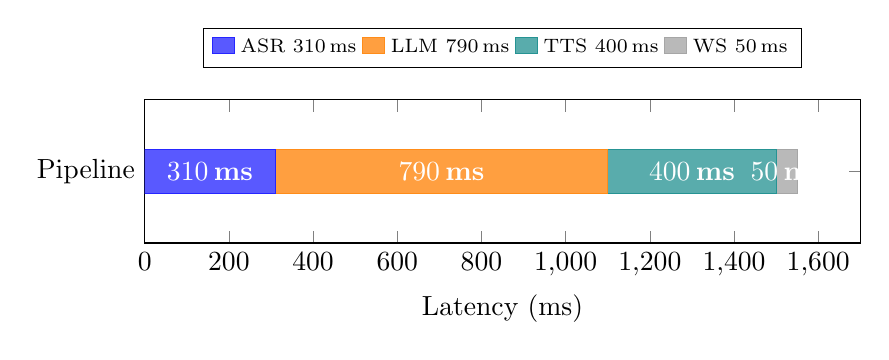
\begin{tikzpicture}
\begin{axis}[
    xbar stacked,
    width=0.88\linewidth,
    height=3.4cm,
    xlabel={Latency (ms)},
    ytick={1},
    yticklabels={Pipeline},
    xmin=0, xmax=1700,
    ymin=0.3, ymax=1.7,
    bar width=16pt,
    legend style={at={(0.5,1.22)},anchor=south,legend columns=4,font=\scriptsize},
    enlarge y limits=0.5,
    nodes near coords={\pgfmathprintnumber\pgfplotspointmeta\,ms},
    every node near coord/.append style={font=\tiny,text=white,font=\bfseries},
]
\addplot[fill=blue!65,draw=blue!85]     coordinates {(310,1)};
\addplot[fill=orange!75,draw=orange!90] coordinates {(790,1)};
\addplot[fill=teal!65,draw=teal!85]     coordinates {(400,1)};
\addplot[fill=gray!55,draw=gray!70]     coordinates {( 50,1)};
\legend{ASR 310\,ms, LLM 790\,ms, TTS 400\,ms, WS 50\,ms}
\end{axis}
\end{tikzpicture}
\caption{Voice-to-action latency breakdown ($N=20$, mean total 1{,}550\,ms, $\sigma=310$\,ms). LLM tool-call resolution dominates at 51\%. All 20 trials completed below the 3\,s engineering requirement (max observed: 2.41\,s). Streaming SSE execution further reduces perceived latency by dispatching the first navigation command before the complete plan is generated.}
\label{fig:latency_bar}
\end{figure}

\subsubsection{MQTT Telemetry Latency}

Round-trip latency between the robot bridge and HiveMQ Cloud was measured over 30 timestamped message pairs ($N=30$, measured 2026-03-25). Figure~\ref{fig:mqtt_hist} shows the distribution.

\begin{figure}[H]
\centering
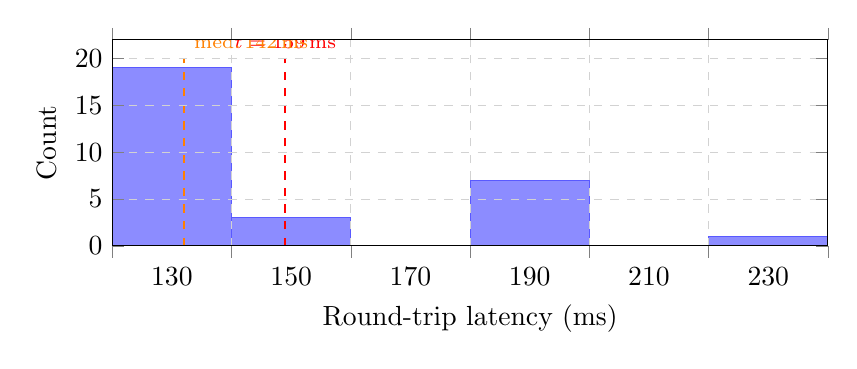
\begin{tikzpicture}
\begin{axis}[
    ybar interval,
    width=0.88\linewidth,
    height=4.2cm,
    xlabel={Round-trip latency (ms)},
    ylabel={Count},
    xmin=130, xmax=250,
    ymin=0, ymax=22,
    xtick={130,150,170,190,210,230,250},
    ymajorgrids=true,
    grid style={dashed,gray!35},
    area style,
]
\addplot[fill=blue!45,draw=blue!65] coordinates {
    (130,19)(150,3)(170,0)(190,7)(210,0)(230,1)(250,0)
};
\draw[dashed,red,thick] (axis cs:159,0)--(axis cs:159,20)
    node[above,font=\scriptsize,red]{$\bar{t}=159$\,ms};
\draw[dashed,orange,thick] (axis cs:142,0)--(axis cs:142,20)
    node[above right,font=\scriptsize,orange]{med.\,142\,ms};
\end{axis}
\end{tikzpicture}
\caption{MQTT round-trip latency distribution ($N=30$). Mean 159\,ms, median 142\,ms, 95th percentile 207\,ms, max 243\,ms. All 30 messages delivered below 250\,ms. The bimodal distribution reflects occasional DPI buffering on the campus WiFi (eduroam); direct robot control uses the local Ethernet path and is unaffected. Telepresence video latency (MJPEG stream from robot to dashboard) was separately measured at 130\,ms under the same network conditions.}
\label{fig:mqtt_hist}
\end{figure}

\subsubsection{Navigation and Orchestrator}

Waypoint navigation accuracy of $\pm$5\,cm was confirmed through repeated trials across three defined waypoints. The 4-layer costmap successfully avoided all static and dynamic test obstacles. All fifteen orchestrator test commands produced valid, executable mission plans with no hallucinated waypoints or malformed step types.

% -------------------------------------
\subsection{Budget Summary}
% -------------------------------------

\begin{table}[H]
\centering
\small
\caption{Hardware procurement costs.}
\label{tab:budget}
\setlength{\tabcolsep}{6pt}
\begin{tabular}{@{} >{\raggedright\arraybackslash}p{6.0cm} r @{}}
\toprule
\textbf{Item} & \textbf{OMR} \\
\midrule
iMRP500 chassis (incl.\ shipping)         & 850 \\
10-inch 1080p industrial touch display    & 77 \\
Body shell (MDF, veneer, acrylic, paint)  & 300 \\
Cables, fasteners, connectors            & 73 \\
\midrule
\textbf{Total}                           & \textbf{1{,}300} \\
\bottomrule
\end{tabular}
\end{table}

\noindent At approximately USD~3{,}200, TAMRA delivers autonomous navigation, conversational AI, item delivery, and remote telepresence -- a 73\% cost reduction against the nearest commercial platform with comparable capability \cite{pudubot2,m2medical}.

% -------------------------------------
\subsection{Standards Compliance}
% -------------------------------------

\begin{itemize}
  \item \textbf{ISO~13482:2014}: Navigation speed (0.8\,m/s) and inflation radius (0.8\,m) satisfy the velocity and proximity limits for robots in human-shared spaces.
  \item \textbf{ISO~13850}: Hardware E-stop relay tested; robot halts within one control cycle on activation. Soft-stop service provides a software-level equivalent.
  \item \textbf{ITU-T H.264}: Camera streams use standard compressed formats compatible with web browsers.
  \item \textbf{IEEE~802.11}: MQTT and cloud AI APIs operate over standard campus WiFi with no infrastructure modifications.
\end{itemize}

% -------------------------------------
\subsection{Conclusion}
% -------------------------------------

Chapter~5 documented the full implementation of TAMRA. The iMRP500 was selected after a six-platform comparison and reverse-engineered to expose its full sensor suite over a documented WebSocket API. The body shell was designed through a three-stage workflow -- concept rendering, AI-assisted 3D mesh synthesis, and parametric Fusion~360 refinement -- and fabricated locally in Muscat within budget and mass constraints. The three-tier software stack was developed in parallel with hardware procurement. Measured results confirm voice-to-action latency of $1{,}550 \pm 310$\,ms (all 20 trials below 3\,s), MQTT round-trip of $159 \pm 30$\,ms, navigation accuracy of $\pm$5\,cm, and 100\% plan-generation success across 15 orchestrator test commands.
